\documentclass[11pt,a4paper]{ctexart}

\usepackage[margin=2.6cm]{geometry}
\usepackage{amsmath,amssymb,amsthm}
\usepackage{graphicx}
\usepackage{booktabs}
\usepackage{hyperref}
\usepackage{xcolor}
\usepackage{listings}
\usepackage{caption}

\graphicspath{{figures/}}
\hypersetup{colorlinks=true, linkcolor=blue!50!black, urlcolor=blue!60!black}
\lstset{
  basicstyle=\ttfamily\small,
  breaklines=true,
  frame=single,
  columns=fullflexible,
  backgroundcolor=\color{gray!7}
}

\newtheorem{definition}{定义}[section]
\newtheorem{theorem}{定理}[section]
\newtheorem{lemma}{引理}[section]
\newtheorem{proposition}{命题}[section]
\newtheorem{example}{例}[section]

\title{第 7 章 \quad Prediction / 预测}
\author{基于 \textit{A Course in Time Series Analysis} 的中文讲义与 Python 实践}
\date{}

\begin{document}
\maketitle

\section*{本章学习目标}

本章按照原文 \textit{Prediction} 的小节顺序整理，保留主要定义、定理、模型公式和练习方向，并将原文中的 R 实践思路改写为 Python 工程实践。

完成本章后，应能够：
\begin{itemize}
  \item 理解预测在估计和模型诊断中的作用；
  \item 推导 AR 与 ARMA 的一步和多步预测；
  \item 掌握有限过去预测与 Durbin-Levinson 递推；
  \item 理解 Kalman 滤波的状态空间预测形式；
  \item 了解非线性模型、Wold 分解和 Kolmogorov 公式。
\end{itemize}

\section{预测在估计中的作用}

预测的目标是在给定信息集 \(\mathcal F_t\) 下预测未来 \(X_{t+h}\)。均方误差意义下的最优预测是条件期望：
\[
  \hat X_{t+h|t}=E(X_{t+h}\mid\mathcal F_t).
\]
若只允许线性预测，则最优预测是向由过去观测张成的线性空间做正交投影。

\section{自回归过程预测}

AR(1)
\[
  X_t=\phi X_{t-1}+\varepsilon_t
\]
的一步预测为
\[
  \hat X_{t+1|t}=\phi X_t,
\]
h 步预测为
\[
  \hat X_{t+h|t}=\phi^hX_t.
\]
预测误差方差为
\[
  \mathrm{var}(X_{t+h}-\hat X_{t+h|t})
  =\sigma^2\sum_{j=0}^{h-1}\phi^{2j}.
\]

\section{AR(p) 与一般时间序列预测}

对 AR(p)，一步预测为
\[
  \hat X_{t+1|t}=\phi_1X_t+\cdots+\phi_pX_{t+1-p}.
\]
多步预测可递归计算：未来尚未观测的 \(X\) 用其预测值代替。

\begin{lemma}[因果 AR(p) 预测，原文 Lemma 7.3.1]
若 \(X_t\) 有因果 AR(p) 表示，则基于无限过去的一步预测由 AR 递推直接给出，预测误差为创新 \(\varepsilon_{t+1}\)。
\end{lemma}

对一般线性过程
\[
  X_t=\sum_{j=0}^{\infty}\psi_j\varepsilon_{t-j},
\]
若创新可由过去观测恢复，则 h 步预测保留已知创新项、舍去未来创新项：
\[
  \hat X_{t+h|t}=\sum_{j=h}^{\infty}\psi_j\varepsilon_{t+h-j}.
\]

\section{有限过去预测与 Durbin-Levinson}

实际中只能使用有限过去 \(X_1,\ldots,X_n\)。最佳线性预测系数由 Toeplitz 正规方程决定。Durbin-Levinson 算法利用 Toeplitz 结构递推求解，大幅降低计算量。

\subsection{Levinson-Durbin 算法}

记 \(\phi_{n,j}\) 为用 \(X_n,\ldots,X_1\) 预测 \(X_{n+1}\) 的系数，\(\phi_{n,n}\) 同时是 n 阶 PACF。递推核心是用上一阶预测误差更新当前阶预测误差。

\subsection{有限与无限预测比较}

原文引入 Baxter 不等式说明：在适当可和条件下，有限过去预测系数会接近无限过去预测系数。这为使用有限样本近似理论预测提供保证。

\section{ARMA、Kalman 滤波与非线性预测}

ARMA 预测可通过创新算法或状态空间形式实现。状态空间模型写作
\[
  \alpha_{t+1}=F\alpha_t+G\varepsilon_{t+1},\qquad
  X_t=H\alpha_t.
\]
Kalman 滤波递推更新状态预测和误差协方差，适合处理缺失观测、多变量和更复杂的动态结构。

非线性模型中，ARCH(p) 和 GARCH(1,1) 的重点是预测条件方差。例如 GARCH(1,1)
\[
  X_t=\sigma_tZ_t,\qquad
  \sigma_t^2=\omega+\alpha X_{t-1}^2+\beta\sigma_{t-1}^2.
\]
其下一期波动率预测为
\[
  \hat\sigma_{t+1}^2=\omega+\alpha X_t^2+\beta\sigma_t^2.
\]

\section{Wold 分解与 Kolmogorov 公式}

\begin{theorem}[Wold 分解，原文 Theorem 7.12.1]
任何零均值、有限方差的二阶平稳过程都可分解为确定性部分和不可预测创新驱动的线性部分。纯非确定性部分可写成
\[
  X_t=\sum_{j=0}^{\infty}\psi_j\varepsilon_{t-j}.
\]
\end{theorem}

Kolmogorov 公式把最小预测误差方差与谱密度联系起来，说明频域结构也决定可预测性。

\section{原文小节覆盖补充}

\subsection{用预测辅助估计}
预测不仅是应用目标，也是估计工具。许多参数可通过最小化一步预测误差平方和估计，这与条件最小二乘和创新算法直接相关。

\subsection{年度温度预测和太阳黑子练习}
第 7.4.1 节用年度温度数据展示实际预测流程：估计趋势或相关结构、生成预测、检查预测误差。Exercise 7.1 要求分析太阳黑子数据并比较预测效果。

\subsection{有限过去一步预测}
有限过去预测使用
\[
  \hat X_{n+1}=\sum_{j=1}^n\phi_{n,j}X_{n+1-j}.
\]
Levinson-Durbin 算法递推求解系数和预测误差方差。Exercise 7.2 要求对 AR(1) 手算该算法。

\subsection{Durbin-Levinson 证明与 Cholesky 分解}
第 7.5.2 从投影几何证明递推；第 7.5.3 说明同一递推可得到 Toeplitz 协方差矩阵的 Cholesky 分解。

\begin{theorem}[Baxter 不等式，原文 Theorem 7.6.1]
若 AR(\(\infty\)) 系数满足适当可和条件，则有限过去预测系数与无限过去预测系数之间的差由尾部系数控制。
\end{theorem}

\subsection{r 步、ARMA 和 Kalman 预测}
r 步预测递归使用未来预测值。ARMA 预测可通过创新递推或状态空间模型实现。第 7.9 节给出 Kalman filter、ARMA 的 Markov 表示和滤波预测公式。

\begin{proposition}[ARMA 预测，原文 Proposition 7.8.1]
若 ARMA 模型因果可逆，则预测误差可由未来创新的线性组合表示，预测误差方差由相应系数平方和给出。
\end{proposition}

\subsection{非线性、非参数、Wold 和 Kolmogorov}
ARCH/GARCH 预测条件方差，双线性模型需要非线性条件期望，非参数预测估计未知回归函数。Wold 分解和 Kolmogorov 公式说明可预测性由创新部分和谱密度共同决定。Exercise 7.3 和 Exercise 7.4 分别对应 GARCH 软件实践和随机周期过程。

\begin{lemma}[附录预测系数，原文 Lemma 7.14.1--7.14.2]
附录控制 AR(p) 预测系数矩阵和谱密度有界时协方差矩阵特征值，为有限预测理论提供技术基础。
\end{lemma}

\section{Python 工程实践}

在本章目录下运行：
\begin{lstlisting}[language=bash]
python scripts/ch07_generate_figures.py
\end{lstlisting}

脚本会把图像写入本章 \texttt{figures/} 目录。当前图像用于配合本章核心概念的仿真说明；若后续补齐原始数据文件，可把模拟数据替换为原文真实数据案例。

\begin{figure}[htbp]
  \centering
  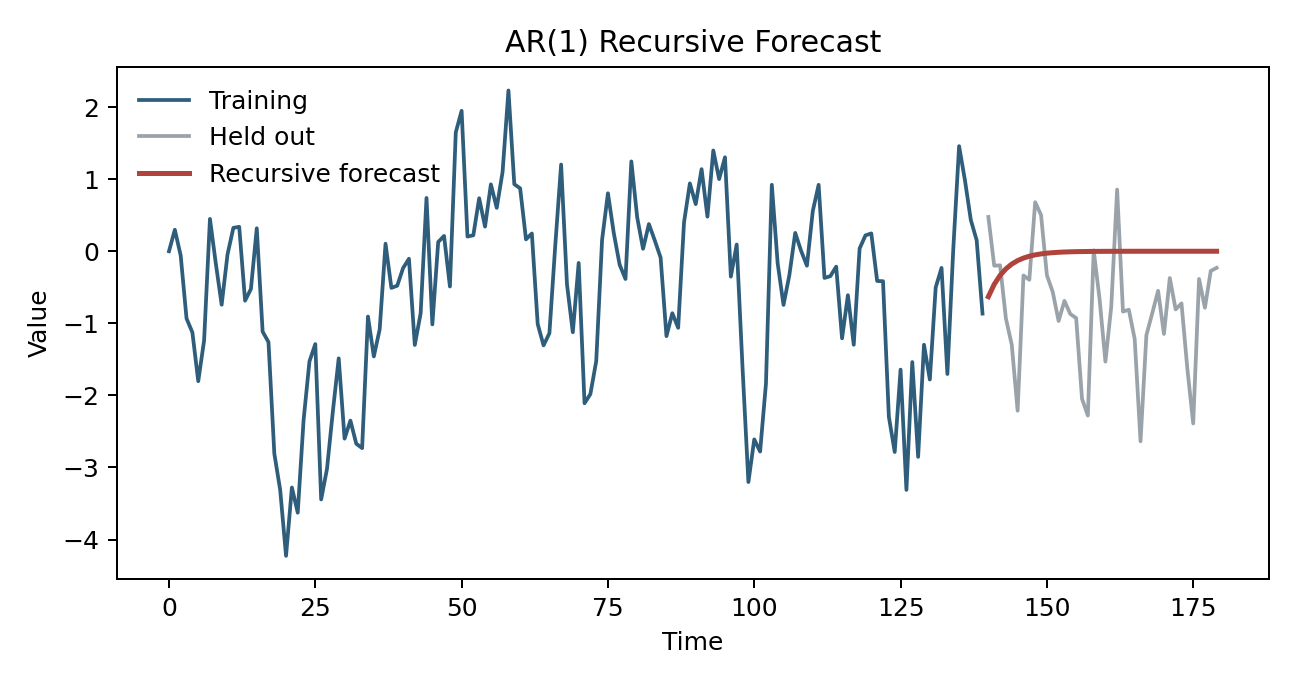
\includegraphics[width=0.86\textwidth]{ch07_fig01_ar_forecast.png}
  \caption{AR(1) 递归预测：多步预测逐渐回到长期均值。}
\end{figure}

\begin{figure}[htbp]
  \centering
  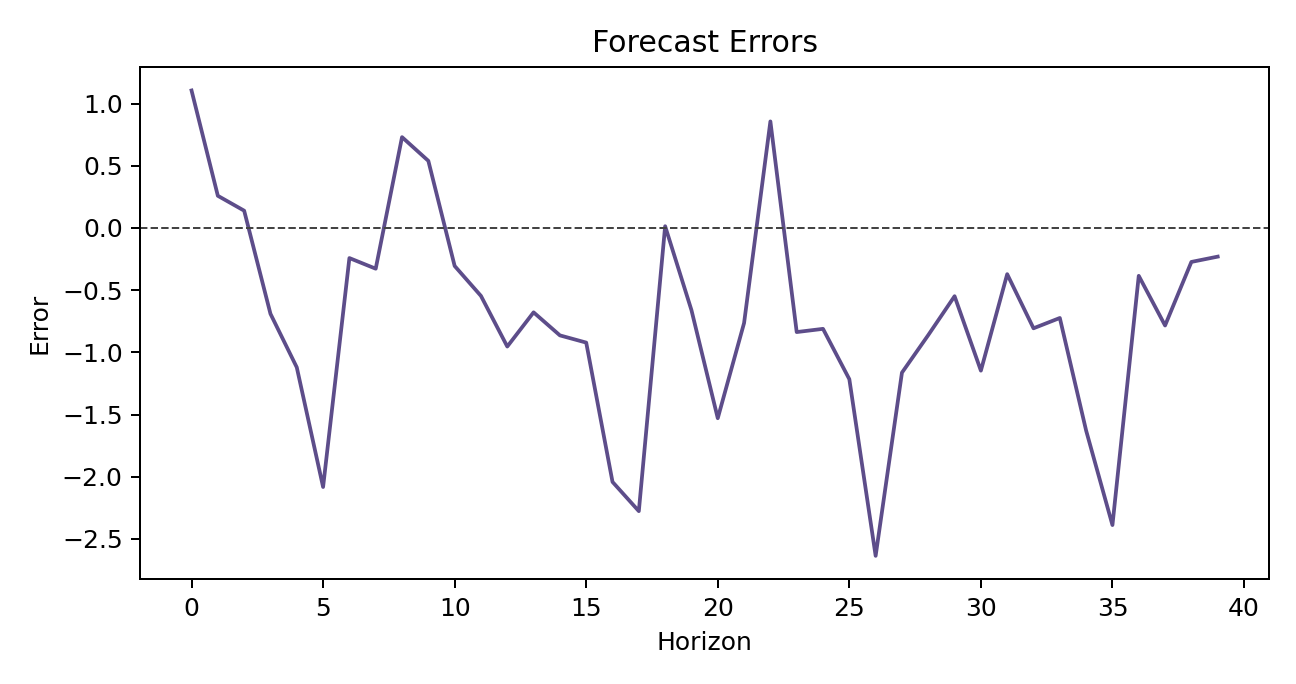
\includegraphics[width=0.86\textwidth]{ch07_fig02_forecast_errors.png}
  \caption{预测误差序列：用于检查预测是否存在系统性偏差或残余相关。}
\end{figure}

\section{练习提要}

原文练习主要围绕下列方向展开：
\begin{itemize}
  \item 用 AR(1) 和 AR(p) 公式计算一步、多步预测；
  \item 手算 Durbin-Levinson 递推的前几阶；
  \item 对太阳黑子或温度数据做预测并比较误差；
  \item 推导 ARCH/GARCH 条件方差预测。
\end{itemize}

\section*{本章小结}

第 7 章把投影理论落实为预测算法。AR 预测可递归计算，有限过去预测由 Durbin-Levinson 高效求解，ARMA 可放入 Kalman 滤波框架，非线性模型则常以条件方差预测为核心。

\end{document}
